

\chapter{Schéma zapojení inerciální jednotky} \label{schemaApp}
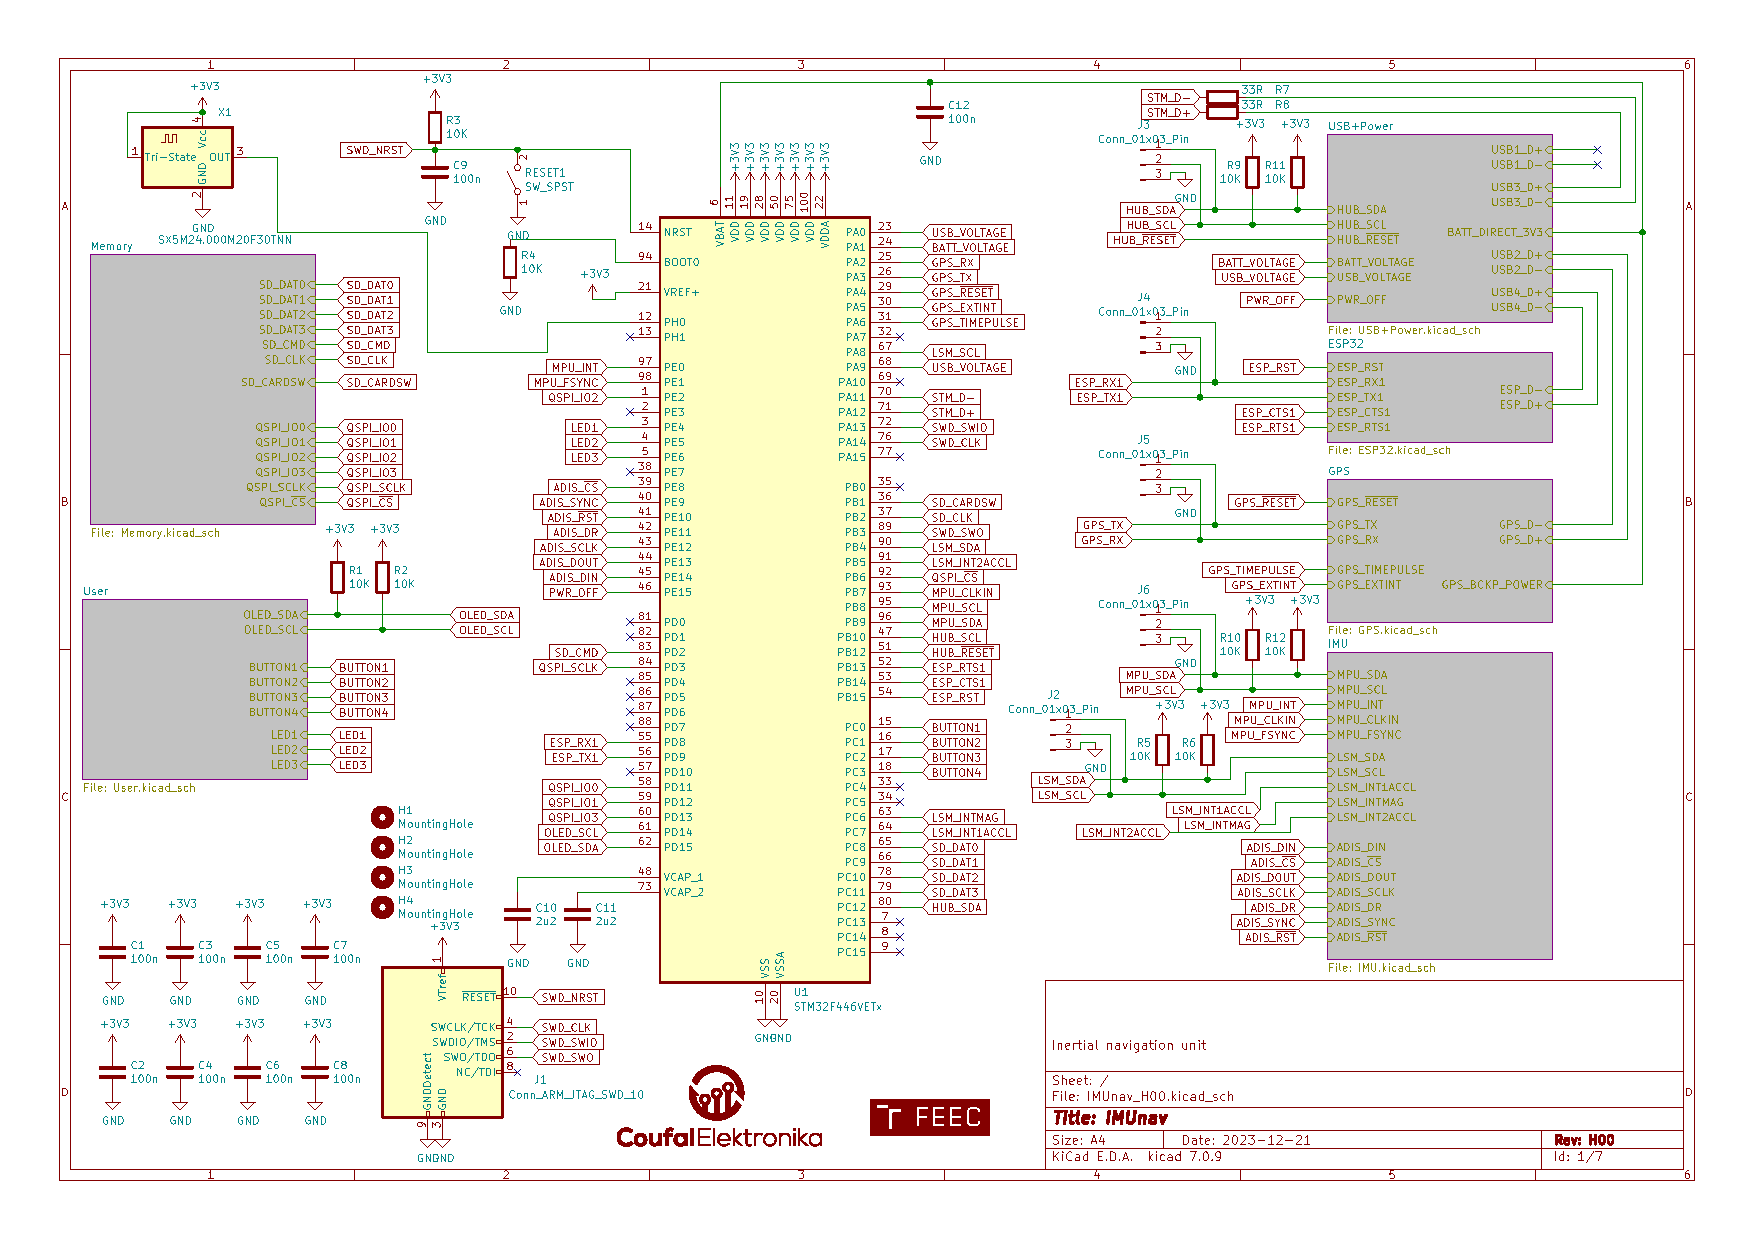
\includegraphics[angle=90, page=1, width=\textwidth]{KiCad/schematic.pdf}

\includegraphics[angle=90, page=2, width=\textwidth]{KiCad/schematic.pdf}

\includegraphics[angle=90, page=3, width=\textwidth]{KiCad/schematic.pdf}

\includegraphics[angle=90, page=4, width=\textwidth]{KiCad/schematic.pdf}

\includegraphics[angle=90, page=5, width=\textwidth]{KiCad/schematic.pdf}

\includegraphics[angle=90, page=6, width=\textwidth]{KiCad/schematic.pdf}

\includegraphics[angle=90, page=7, width=\textwidth]{KiCad/schematic.pdf}

\chapter{Výkres DPS}
\section{Pohled osazení součástek} \label{placementApp}
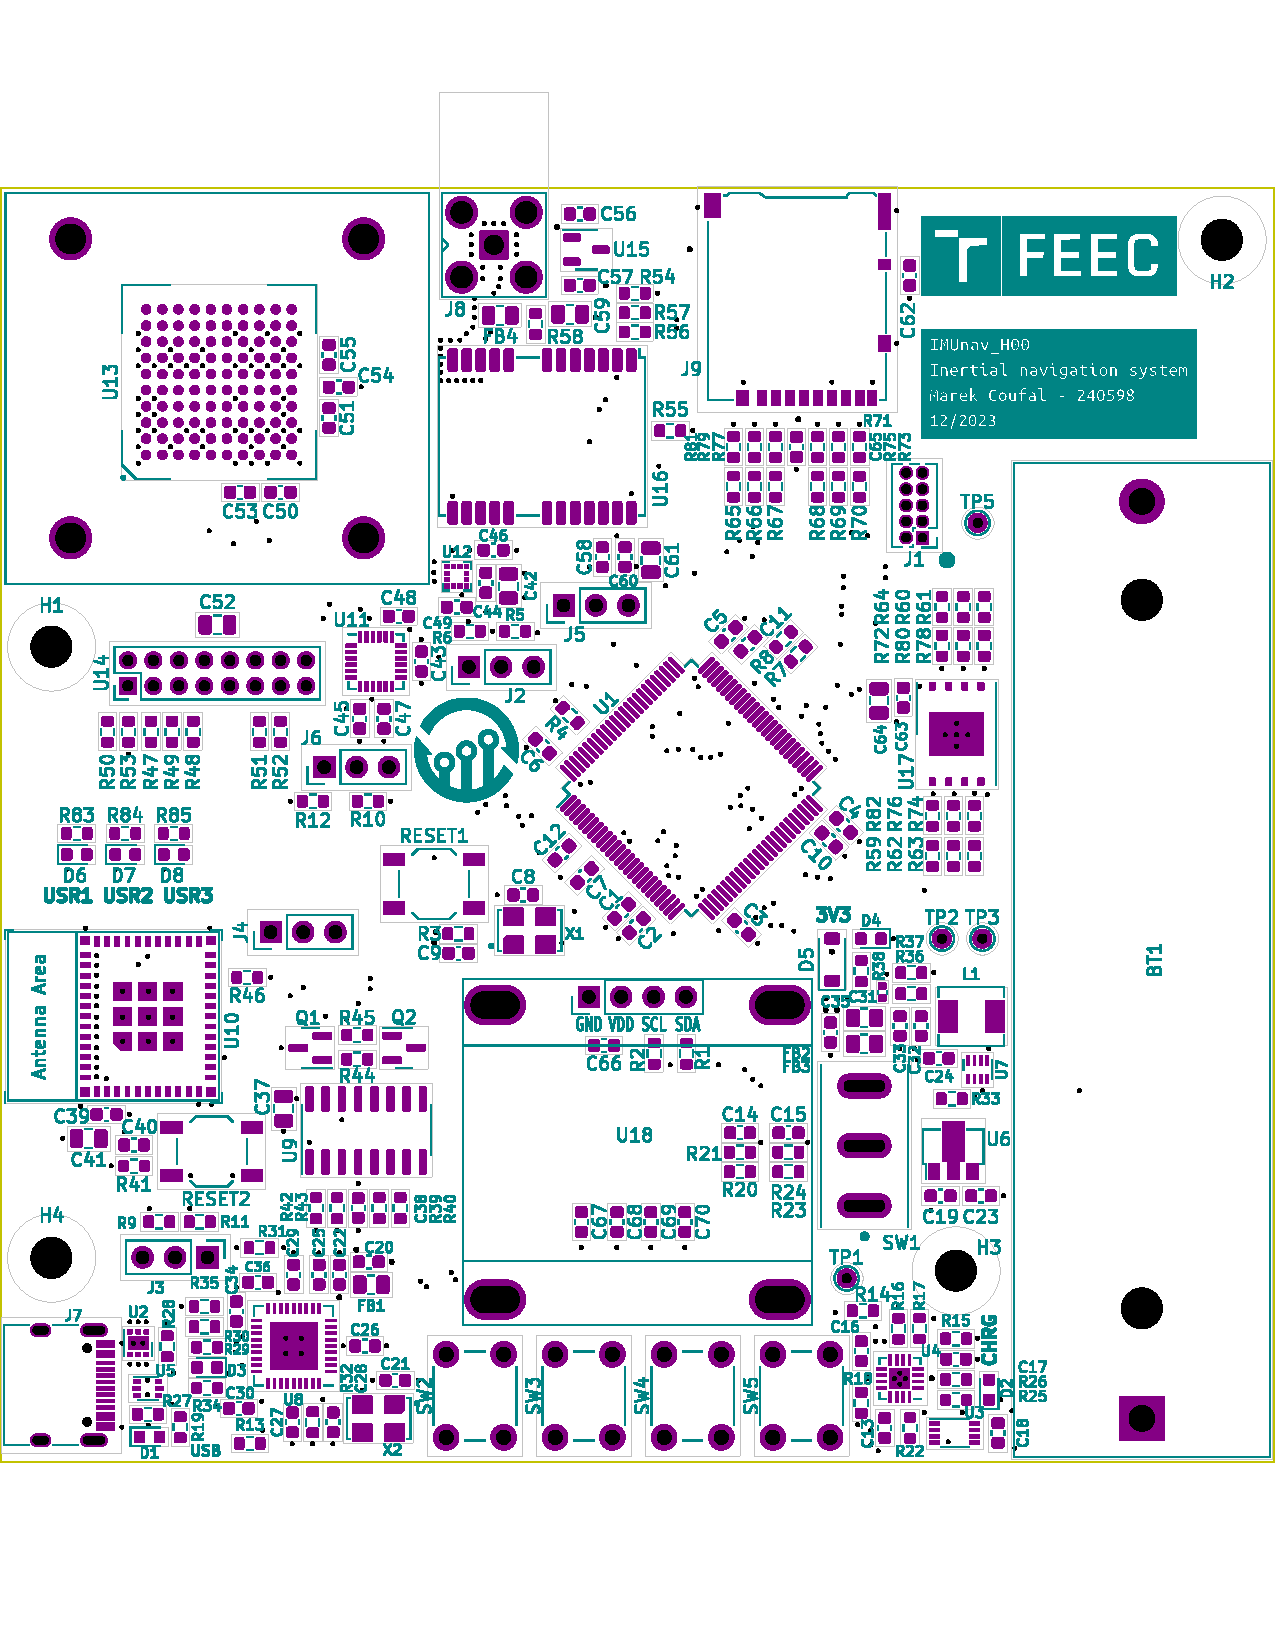
\includegraphics[width=\textwidth]{KiCad/boardTopParts}

\section{Vrchní vrstva mědi DPS} \label{TopApp}
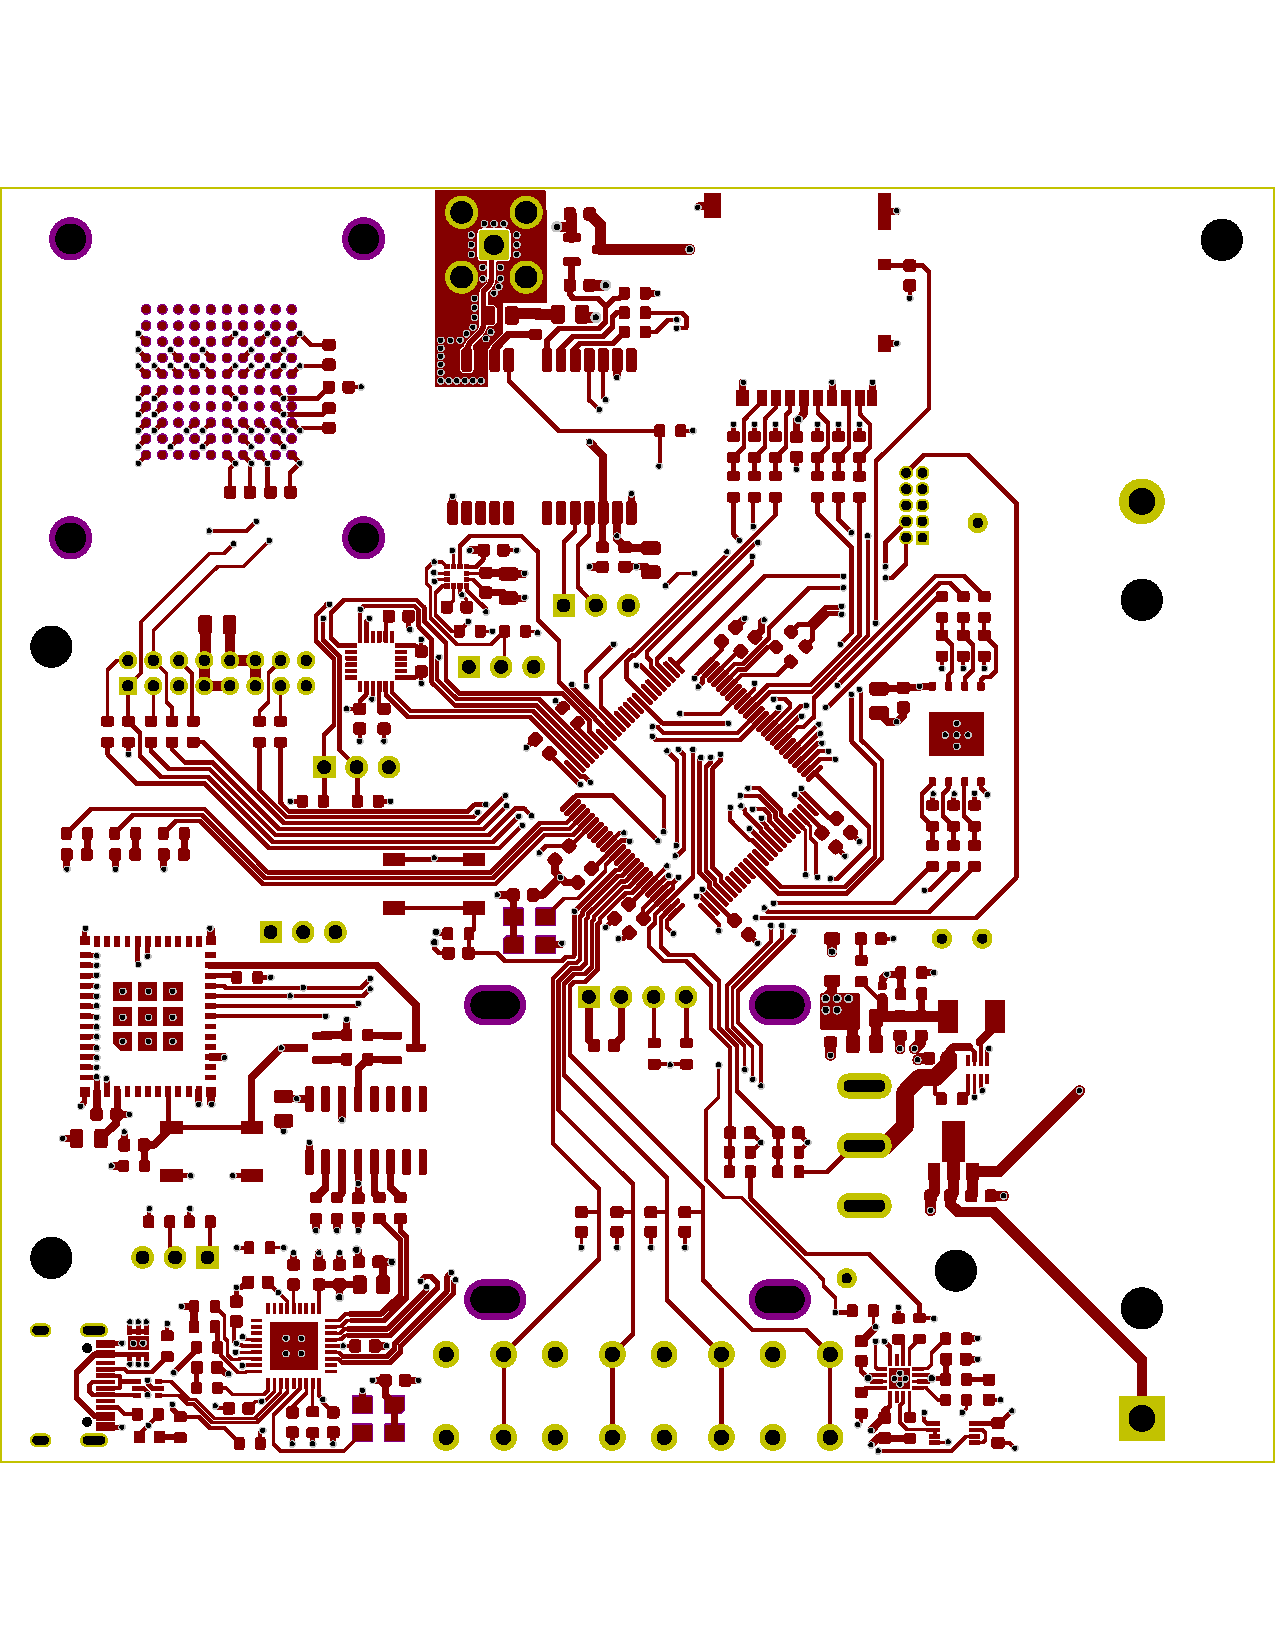
\includegraphics[width=\textwidth]{KiCad/boardF}

\section{Vnitřní vrstva mědi DPS In1}
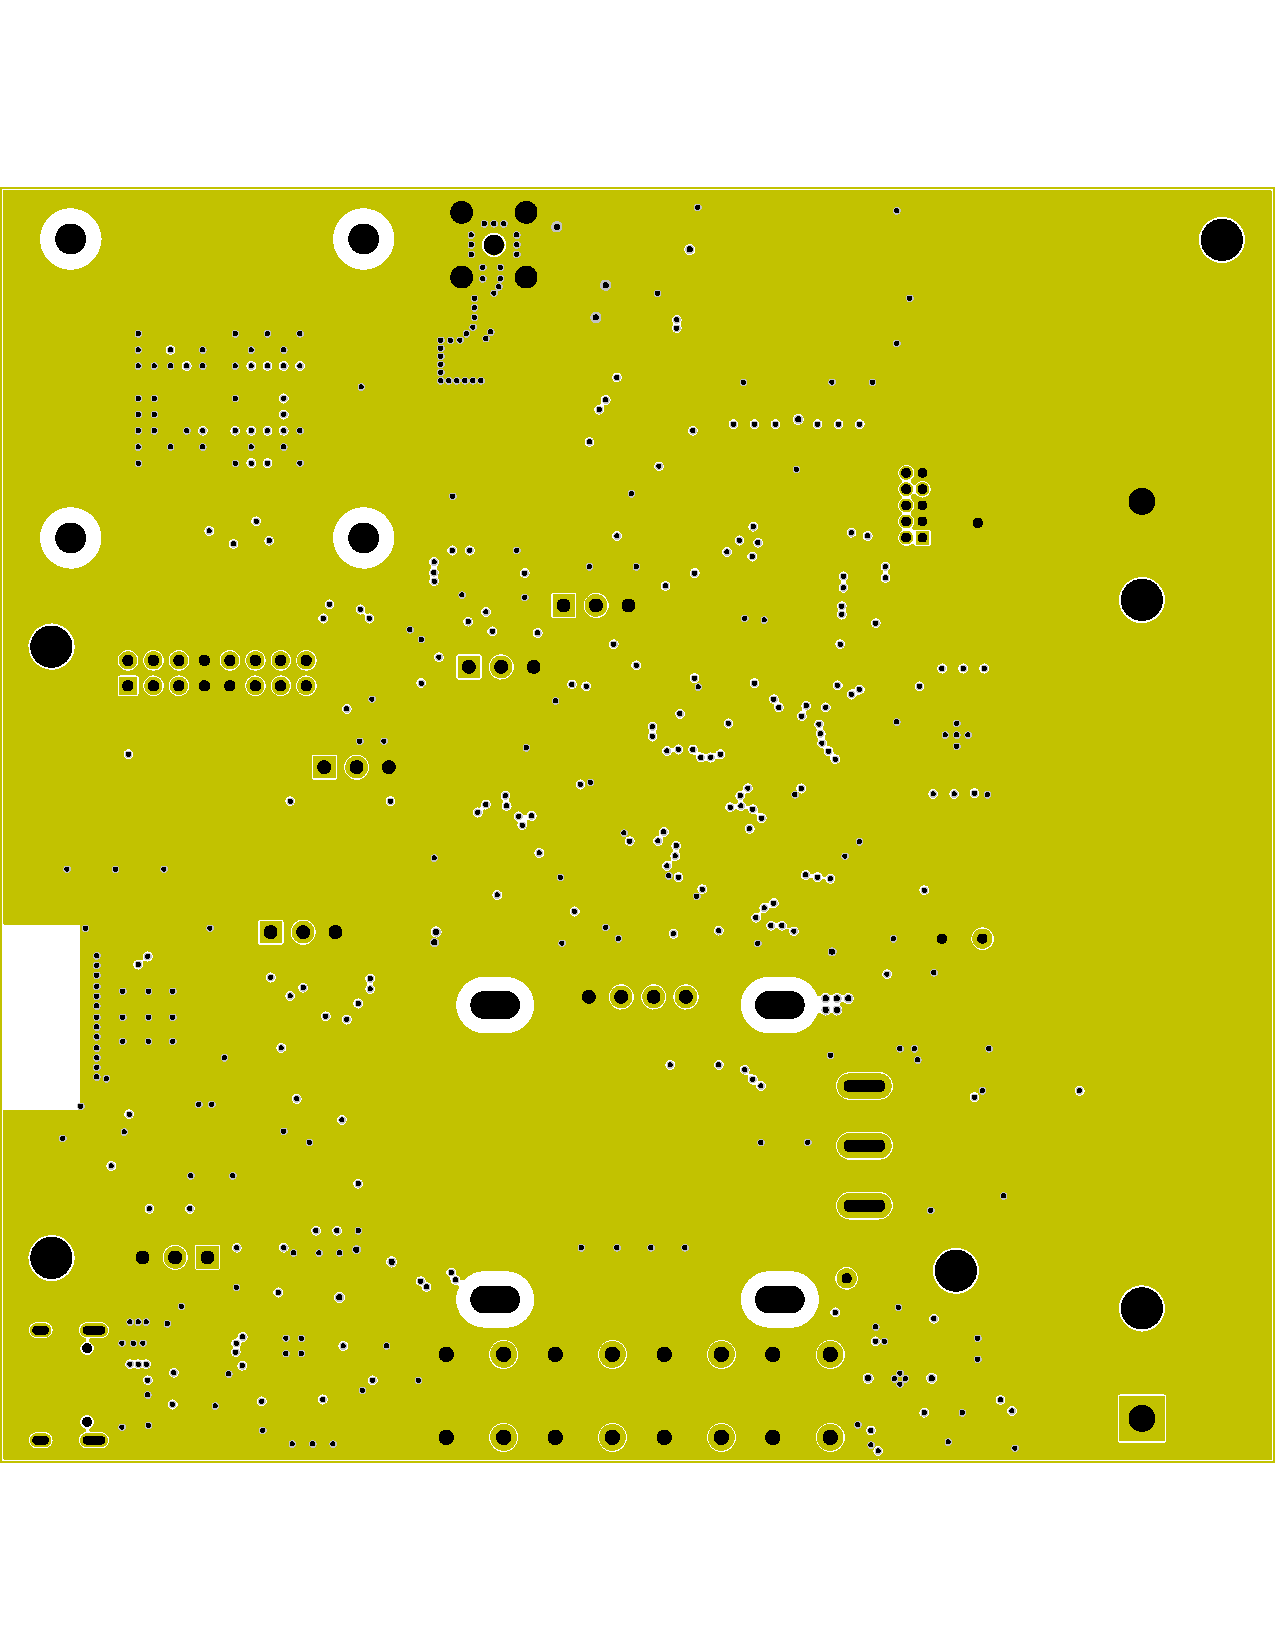
\includegraphics[width=\textwidth]{KiCad/boardIn1}

\section{Vnitřní vrstva mědi DPS In2}
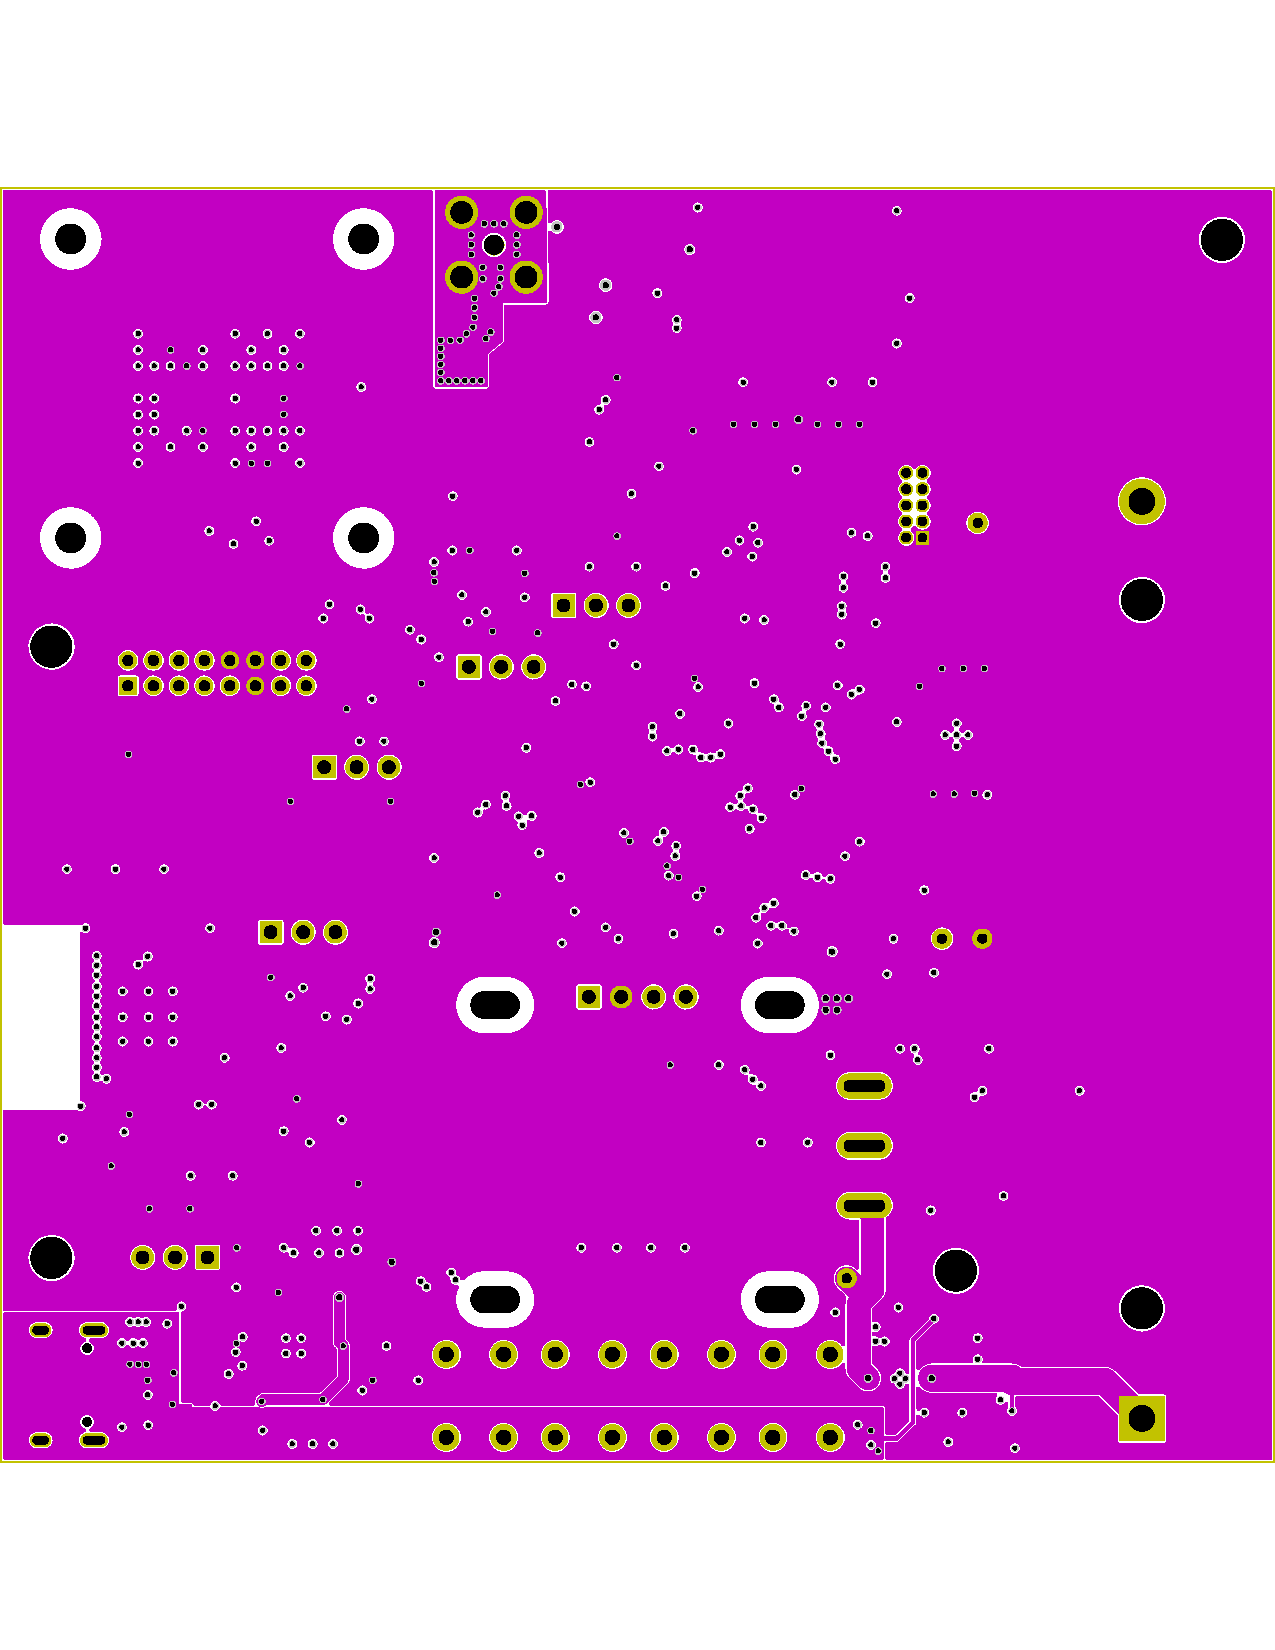
\includegraphics[width=\textwidth]{KiCad/boardIn2}

\section{Spodní vrstva mědi DPS} \label{BottomApp}
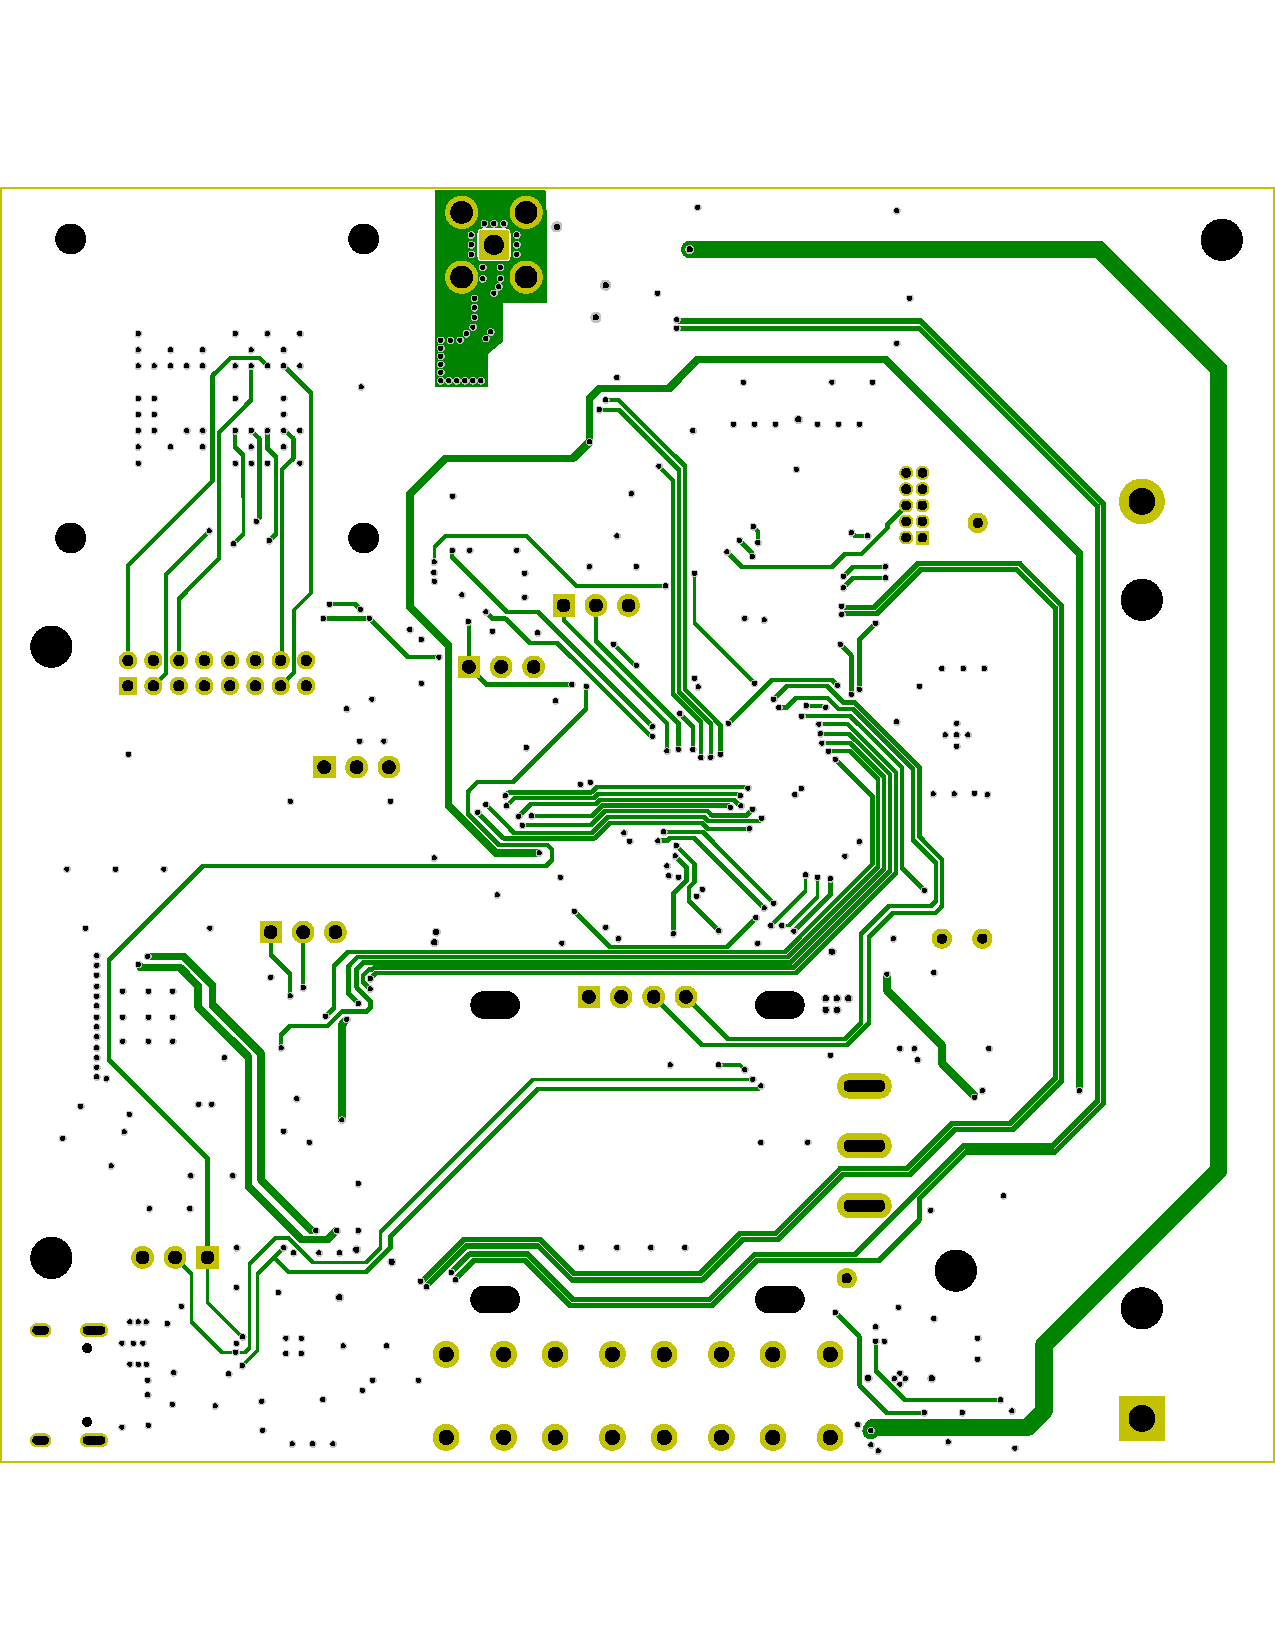
\includegraphics[width=\textwidth]{KiCad/boardB}


\chapter{Obsah elektronické přílohy}

\dirtree{%
 .1 .
 .2 Firmware.
 .3 IMUnav\_STM\_F00\DTcomment{složka projektu Firmwaru MCU}. 
 .4 Core.
 .5 AccelCalSolver\DTcomment{vygenerované soubory kalibrační procedury}.
 .6 \dots.
 .5 Inc\DTcomment{hlavičkové soubory}.
 .6 \dots.
 .5 Src\DTcomment{zdrojové soubory}.
 .6 \dots.
 .4 Debug.
 .5 \dots.
 .4 Drivers\DTcomment{HAL knihovny}.
 .5 \dots.
 .4 FATFS\DTcomment{knihovna souborového systému}.
 .5 \dots.
 .4 Middlewares\DTcomment{zdrojové soubory pro FatFS, USB a FreeRTOS}.
 .5 \dots.
 .4 Release.
 .5 \dots.
 .4 USB\_DEVICE\DTcomment{knihovna pro USB zařízení}.
 .5 \dots.
 .4 IMUnav\_STM\_F00 Debug.launch.
 .4 IMUnav\_STM\_F00.ioc.
 .4 STM32F446VETX\_FLASH.ld\DTcomment{linker skript pro FLASH}.
 .4 STM32F446VETX\_RAM.ld\DTcomment{linker skript pro RAM}.
 .2 Hardware.
 .3 IMUnav-libra\DTcomment{knihovna součástek a loga}.
 .4 \dots.
 .3 IMUnav\_H00\DTcomment{složka projektu DPS}.
 .4 bom.
 .5 ibom.html\DTcomment{seznam součástek}.
 .4 production.
 .5 \dots.
 .4 ESP32.kicad\_sch\DTcomment{list schématu}.
 .4 GPS.kicad\_sch\DTcomment{list schématu}.
 .4 IMU.kicad\_sch\DTcomment{list schématu}.
 .4 IMU.kicad\_sch-bak.
 .4 IMUnav\_H00.kicad\_dru.
 .4 IMUnav\_H00.kicad\_pcb\DTcomment{deska}.
 .4 IMUnav\_H00.kicad\_prl.
 .4 IMUnav\_H00.kicad\_pro.
 .4 IMUnav\_H00.kicad\_sch\DTcomment{list schématu}.
 .4 IMUnav\_H00.kicad\_sch-bak.
 .4 IMUnav\_H00.step\DTcomment{3D model desky}.
 .4 Memory.kicad\_sch\DTcomment{list schématu}.
 .4 USB+Power.kicad\_sch\DTcomment{list schématu}.
 .4 User.kicad\_sch\DTcomment{list schématu}.
 .4 fp-info-cache.
 .4 fp-lib-table.
 .4 sym-lib-table.
 .2 Software.
 .3 Matlab\DTcomment{složka vytvořených MATLAB skriptů a vzorových dat}.
 .4 C generator\DTcomment{složka kalibrační procedury}.
 .5 \dots.
 .4 IMUonlyNavigation.m\DTcomment{skript pro výpočet trajektorie pomocí pohybových rovnic}.
 .4 chuzePoByte.csv\DTcomment{vzorová data}.
 .4 chuzeVenkuCALB.csv\DTcomment{vzorová data}.
 .4 ctverecChuze.csv\DTcomment{vzorová data}.
 .4 ctverecChuze2.csv\DTcomment{vzorová data}.
 .4 ctverecChuze3CALB.csv\DTcomment{vzorová data}.
 .4 ctverecRychlaChuze.csv\DTcomment{vzorová data}.
 .4 imuAndGnssInsfilterMARG.m\DTcomment{skript pro fúzi dat pomocí Navigation Toolboxu}.
 .4 koleckoKolemFEKTUCALB.csv\DTcomment{vzorová data}.
 .4 tiltedStationary.csv\DTcomment{vzorová data}.
 .3 Python.
 .4 IMUDATA.BIN\DTcomment{vzorová binární data}.
 .4 binDecoder.py\DTcomment{skript pro převod binárních dat na CSV}.
}

